\item \textbf{{[}JPJC/PRELIM/9597/2019/P2/Q8{]} }

An Abstract Data Type (ADT) is a type (or class) for objects whose
behavior is defined by a set of value and a set of operations. 

A linked list ADT has the following operations defined:
\begin{enumerate}
\item[i. ]  \texttt{Create(x)} -- creates an empty linked list \texttt{x}.
\item[ii.]  \texttt{Insert(x,item,i)} -- inserts new value, \texttt{item},
into linked list \texttt{x} so that it is at position \texttt{i} in
the linked list.
\item[iii.]  \texttt{Delete(x,i)} -- deletes the \texttt{item} at position \texttt{i}
in the linked list \texttt{x}.
\item[iv.]  \texttt{Read(x,i)} -- returns the \texttt{item} at position \texttt{i}
in the linked list \texttt{x}.
\item[v.]  \texttt{Length(x)} -- returns the number of items in the linked
list \texttt{x}.
\item[vi.]  \texttt{IsEmptyList(x)} -- returns true if linked list \texttt{x}
is empty.
\end{enumerate}
The linked list is implemented by the use of a collection of nodes
that has \textbf{two} parts: the \textbf{data} and a \textbf{pointer
to the next item} in the linked list. In addition, there is a Start
pointer which points to the first node in the list. 
\begin{enumerate}
\item Assume a node with the following structure: 
\begin{center}
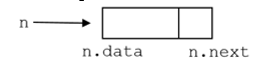
\includegraphics[width=0.25\paperwidth]{C:/Users/Admin/Desktop/Github/question_bank/LyX/static/img/9597-JPJC-2019-P2-Q8-1}
\par\end{center}

Complete the algorithm to implement the 'Delete' operation: \hfill{}{[}5{]}

\noindent %
\noindent\begin{minipage}[t]{1\columnwidth}%
\texttt{PROCEDURE Delete (x, i) }

\texttt{\qquad{}IF Length(x) = 0 THEN }

\texttt{\qquad{}\qquad{}....................................A.................................... }

\texttt{\qquad{}ENDIF }

\texttt{\qquad{}IF i = 1 THEN // situation 1: delete the 1st node }

\texttt{\qquad{}\qquad{}temp <- Start }

\texttt{\qquad{}\qquad{}....................................B.................................... }

\texttt{\qquad{}ELSE // situation 2 : delete middle node }

\texttt{\qquad{}\qquad{}Previous <- NULL }

\texttt{\qquad{}\qquad{}Current <- Start }

\texttt{\qquad{}\qquad{}FOR n <- 1 TO (i \textendash{} 1) STEP 1 }

\texttt{\qquad{}\qquad{}\qquad{}....................................C.................................... }

\texttt{\qquad{}\qquad{}\qquad{}....................................D.................................... }

\texttt{\qquad{}\qquad{}NEXT n }

\texttt{\qquad{}\qquad{}\qquad{}....................................E.................................... //
make the deletion }

\texttt{\qquad{}ENDIF }

\texttt{ENDPROCEDURE }%
\end{minipage}
\item Show how the following operations for an ADT called QUEUE using the
linked list ADT operations can be implemented. 
\begin{enumerate}
\item Create new queue. \hfill{}{[}1{]}
\item Add item to a queue. \hfill{}{[}2{]}
\item Delete item from a queue. \hfill{} {[}2{]}
\end{enumerate}
\end{enumerate}